\subsection{DATOS}
Amplificador Operacional LM324.

V+ = 10V V- = 0V

R1 = R2 = R4 = $10K\Omega$ y R3 = $2K\Omega$

$V_{ref}=2V$

\begin{center}
	\resizebox{8cm}{!}{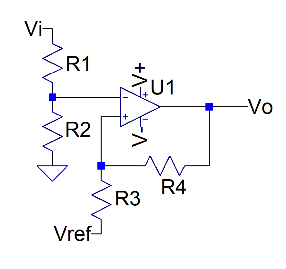
\includegraphics{Imagenes/CIV.png}} \\
	\stepcounter{figure}
	\begin{center}
    	\begin{small}
        \textit{Fig.\thefigure \ - \ 	Circuito IV: Comparador con histéresis.}
		\end{small}
    \end{center}
\end{center}

\subsection{PARÁMETROS/RELACIONES A ANALIZAR:}

\noindent \textbf{ANALÍTICO:}
\begin{enumerate}[4.1]
    \item Umbral de conmutación cuando Vo=V+
    \item Impedancia vista por las fuentes de señal
\end{enumerate}

\subsection{MEDICIÓN - SIMULACIÓN:}
\begin{enumerate}[4.3]
    \item Gráfico Entrada/Salida: $V_{o}=f(V_{i})$\hspace{0.25cm} $V-$ $<V_{C}<$ $V+$
\end{enumerate}
